\documentclass[tikz,border=8pt]{standalone}
\usepackage{amsmath,amssymb}
\usetikzlibrary{arrows.meta,positioning,calc,shapes.geometric}
\tikzset{
  arr/.style={-{Stealth[length=3mm,width=2.4mm]},line width=1.3pt},
  pillar/.style={draw,rounded corners=6pt,fill=blue!20,minimum width=6.2cm,minimum height=2.5cm,align=center,font=\Large,inner sep=6pt},
  note/.style={draw,rounded corners=5pt,fill=gray!12,minimum width=5.8cm,minimum height=1.0cm,align=center,font=\small,inner sep=5pt},
  top/.style={draw,rounded corners=6pt,fill=green!20,minimum width=12.5cm,minimum height=2.3cm,align=center,font=\Large,inner sep=6pt},
}
\begin{document}
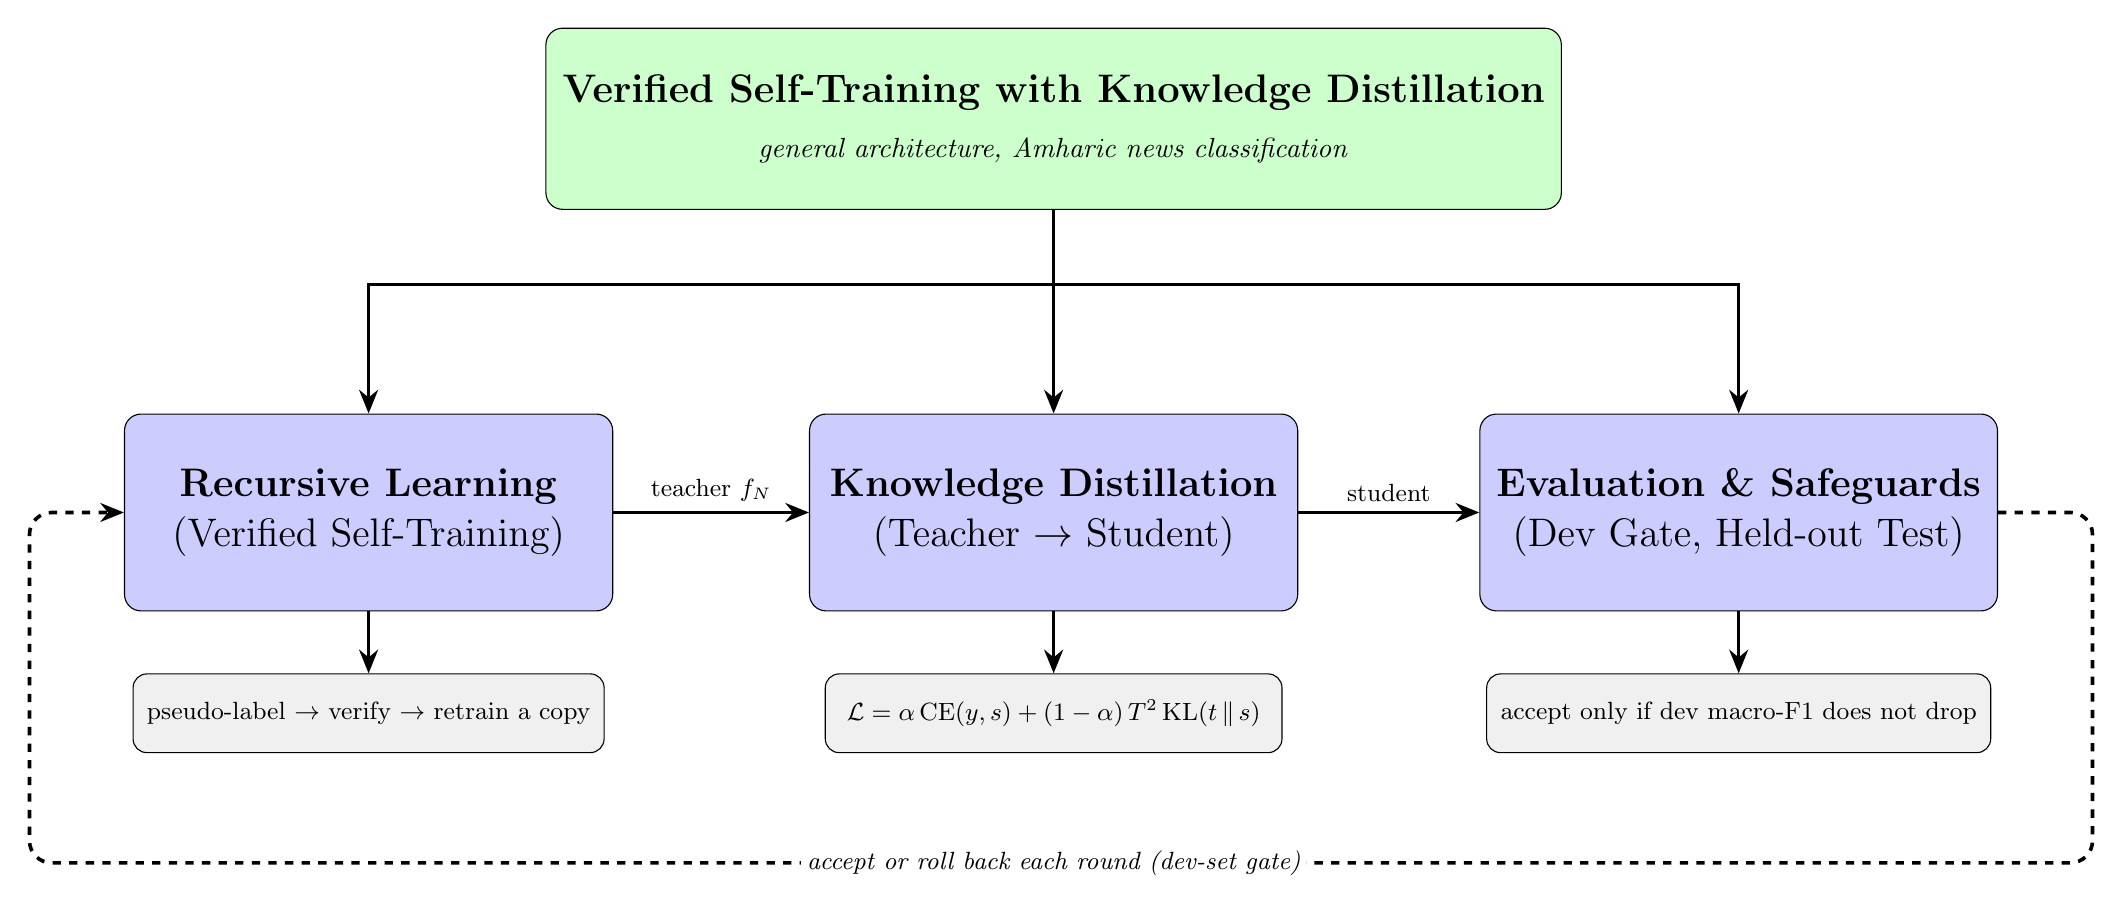
\begin{tikzpicture}
\node[top] (T) at (0,0) {\textbf{Verified Self-Training with Knowledge Distillation}\\[2pt]{\normalsize\textit{general architecture, Amharic news classification}}};
\node[pillar] (A) at (-8.7,-5.0) {\textbf{Recursive Learning}\\(Verified Self-Training)};
\node[pillar] (B) at (0,-5.0) {\textbf{Knowledge Distillation}\\(Teacher $\rightarrow$ Student)};
\node[pillar] (C) at (8.7,-5.0) {\textbf{Evaluation \& Safeguards}\\(Dev Gate, Held-out Test)};
\node[note] (nA) at (-8.7,-7.55) {pseudo-label $\rightarrow$ verify $\rightarrow$ retrain a copy};
\node[note] (nB) at (0,-7.55) {$\mathcal{L}=\alpha\,\mathrm{CE}(y,s)+(1-\alpha)\,T^{2}\,\mathrm{KL}(t\,\|\,s)$};
\node[note] (nC) at (8.7,-7.55) {accept only if dev macro-F1 does not drop};
% top fan-out
\draw[arr] (T.south) -- (B.north);
\draw[arr] (T.south) -- ++(0,-0.95) -| (A.north);
\draw[arr] (T.south) -- ++(0,-0.95) -| (C.north);
% pillars to notes
\draw[arr] (A.south) -- (nA.north);
\draw[arr] (B.south) -- (nB.north);
\draw[arr] (C.south) -- (nC.north);
% data flow between pillars
\draw[arr] (A.east) -- node[above,font=\small] {teacher $f_N$} (B.west);
\draw[arr] (B.east) -- node[above,font=\small] {student} (C.west);
% feedback loop (dev gate) routed around the bottom
\draw[arr,dashed,rounded corners=8pt] (C.east) -- ++(1.2,0) |- (0,-9.45) -| ([xshift=-1.2cm]A.west) -- (A.west);
\node[fill=white,inner sep=2pt,font=\small\itshape] at (0,-9.45) {accept or roll back each round (dev-set gate)};
\end{tikzpicture}
\end{document}
